\documentclass{ltxdoc}
\usepackage{phd}
\begin{document}
<<<<<<< HEAD
%%%%%%%%%%%%%%%%%%%%%%%%%%%%%%%%%%%%%%%%%%%
%%%%%%  STYLE 10
%%%%%%%%%%%%%%%%%%%%%%%%%%%%%%%%%%%%%%%%%%%

\cxset{
 name=CHAPTER,
 numbering=WORDS,
 number font-size=\huge,
 number font-family=\sffamily,
 number font-weight=\bfseries,
 number before=,
 number dot=,
 number after=\hspace{1em},
 number position=rightname,
 chapter font-family=\sffamily,
 chapter font-weight=\bfseries,
 chapter font-size=\huge,
 chapter before={\vspace*{0.4\textheight}\hfill},
 chapter after={\hfill\hfill\vskip0pt\thinrule\par},
 chapter color={black!90},
 number color=\color{black!90},
 title beforeskip={\vspace*{30pt}},
 title afterskip={\vspace*{30pt}\par},
 title before={\hfill},
 title after={\hfill\hfill},
 title font-family=\sffamily,
 title font-color=\color{black!90},
 title font-weight=\bfseries,
 title font-size=\huge,
 section font-size=\LARGE,
 section font-weight=\normalfont,
 section font-family=\sffamily,
 section align=,
 section numbering=none,
 section indent=-1em,
 section align=\centering,
 section beforeskip=20pt,
 section afterskip=10pt,
 section spaceout=soul,
 section font-shape=,
}

 %set the sectioning commands


\renewsection

\chapter{INTRODUCTION TO STYLE TEN}

\section{Basic Description:}
This chapter style has the unique characteristic that the chapter number is spelled out, rather than being in arabic numerals. The setting for this is the option \lstinline{numeric=WORDS}. Use either a capital for uppercase or \lstinline{numeric=words} for lowercase number labels.

\medskip
\begin{figure}[ht]
\centering
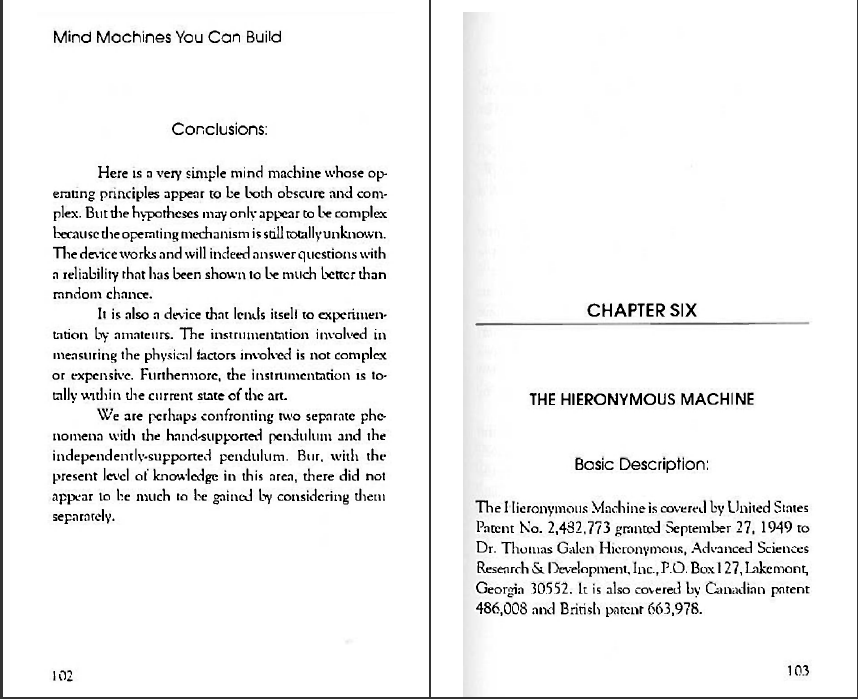
\includegraphics[width=0.6\textwidth]{./chapters/chapter10}
\end{figure}

\lipsum[1]
=======
%%%%%%%%%%%%%%%%%%%%%%%%%%%%%%%%%%%%%%%%%%%
%%%%%%  STYLE 10
%%%%%%%%%%%%%%%%%%%%%%%%%%%%%%%%%%%%%%%%%%%

\cxset{
 name=CHAPTER,
 numbering=WORDS,
 number font-size=\huge,
 number font-family=\sffamily,
 number font-weight=\bfseries,
 number before=,
 number dot=,
 number after=\hspace{1em},
 number position=rightname,
 chapter font-family=\sffamily,
 chapter font-weight=\bfseries,
 chapter font-size=\huge,
 chapter before={\vspace*{0.4\textheight}\hfill},
 chapter after={\hfill\hfill\vskip0pt\thinrule\par},
 chapter color={black!90},
 number color=\color{black!90},
 title beforeskip={\vspace*{30pt}},
 title afterskip={\vspace*{30pt}\par},
 title before={\hfill},
 title after={\hfill\hfill},
 title font-family=\sffamily,
 title font-color=\color{black!90},
 title font-weight=\bfseries,
 title font-size=\huge,
 section font-size=\LARGE,
 section font-weight=\normalfont,
 section font-family=\sffamily,
 section align=,
 section numbering=none,
 section indent=-1em,
 section align=\centering,
 section beforeskip=20pt,
 section afterskip=10pt,
 section spaceout=soul,
 section font-shape=,
}

 %set the sectioning commands


\renewsection

\chapter{INTRODUCTION TO STYLE TEN}

\section{Basic Description:}
This chapter style has the unique characteristic that the chapter number is spelled out, rather than being in arabic numerals. The setting for this is the option \lstinline{numeric=WORDS}. Use either a capital for uppercase or \lstinline{numeric=words} for lowercase number labels.

\medskip
\begin{figure}[ht]
\centering
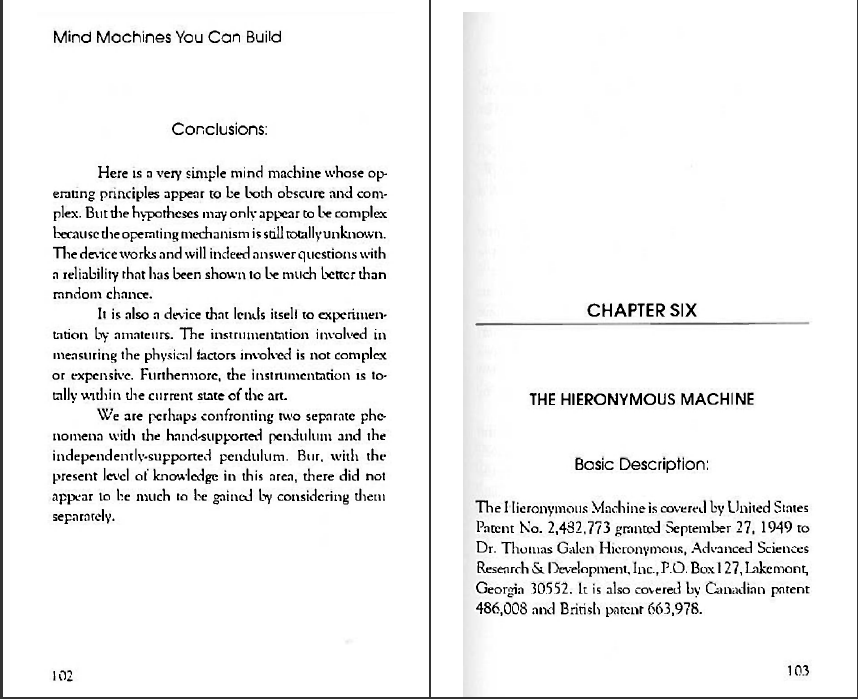
\includegraphics[width=0.6\textwidth]{./chapters/chapter10}
\end{figure}

\lipsum[1]
>>>>>>> merged

\chapter{Iteration}
\index{Iteration}
\index{Iteration!\textbackslash loop}
\index{Iteration!\textbackslash repeat}
\section*{\TeX's simple \protect\texttt{loop}}



\newthought{Knuth in the TeXBook} provided a simple loop macro that can be used for iteration. It must be pointed out that there are no real looping structures in \tex other than pure recursion (including tail recursion). All looping mechanisms are build on top of these.

The |\loop...\repeat| construction is defined in Plain TeX and works like this:
You say `|\loop| $\alpha$ |\if|\dots $\beta$  |\repeat|', where $\alpha$ and $\beta$ are any sequences of
commands, and where |\if...| is any conditional test (without a matching |\fi|). 

\tex
will first do $\alpha$; then if the condition is true, \tex will do $\beta$ and repeat the whole process
again starting with $\alpha$. If the condition ever turns out to be false, the loop will stop.

\emphasis{loop,repeat}
\begin{texexample}{Knuth's Loop}{}
\bgroup
\newcount\n
\n=0
\loop
   \advance\n by1
     \number\n,   
   \ifnum\n<30
\repeat
\egroup
\end{texexample}



%%% This ideally should be in a token register
%%% to modify
{\noindent
\newcount\n
\n=0
\loop%
   \advance\n by1
     \texttt{\number\n, }%  
   \ifnum\n<30%
\repeat%
}

The \cmd{\loop} macro that does all these wonderful things is actually quite simple.
It puts the code that's supposed to be repeated into a control sequence called
\cmd{\body}, and then another control sequence iterates until the condition is false:

\begin{teX}
\def\loop#1\repeat{\def\body{#1}\iterate}
\def\iterate{\body\let\next=\iterate\else\let\next=\relax\fi\next}
\end{teX}


\noindent\colorbox{gray!10}{\parbox{10cm}{\noindent
\newcount\n
\n=0
\loop
   \advance\n by1
     \texttt{\number\n, } 
   \ifnum\n<30
\repeat
}}
\bigskip

Just observe that the |\loop| arguments are delimited by |\repeat|. We could as well named it |\endloop| (a repeat at the end of a loop somehow sounds wrong!)

\emphasis{for,endfor}
\begin{teX}
\def\for#1\endfor{\def\body{#1}\iterate}
\def\iterate{\body\let\next=\iterate\else\let\next=\relax\fi\next}
\newcount\n
\n=0
% Example usage
\for
   \advance\n by1
     \texttt{\number\n, }  
   \ifnum\n<30
\endfor
\end{teX}  

\def\for#1\endfor{\def\body{#1}\iterate}
\def\iterates{\body\let\next=\iterates\else\let\next=\relax\fi\next}

\noindent\colorbox{gray!10}{\parbox{10cm}{\noindent
\newcount\n
\n=0
\for%
   \advance\n by1
     \texttt{\number\n, }%  
   \ifnum\n<30%
\endfor%
}}

\subsection{Breaking out of a loop}

\index{Iteration!break}\index{\protect\textbackslash break}
Although the loop macros are fairly simple, breaking out of them or using conditionals needs some work.

\emphasis{let,iterate,relax}
\begin{teXXX}
\newcount\mycount
\mycount=0
\loop\ifnum\mycount<13
A 
\ifnum\mycount>5
    \let\iterate\relax
 \fi
 \advance\mycount by1\relax
\repeat
\end{teXXX}
\medskip
producing:
\medskip

%\def\graybox#1{%
%\noindent\colorbox{gray!10}{\parbox{10cm}{\noindent#1}}\par\medskip}

\graybox{
\newcount\mycount
\mycount=0
\loop\ifnum\mycount<13
\the\mycount, 
\ifnum\mycount>5
    \let\iterate\relax
 \fi
 \advance\mycount by1\relax
\repeat
}

One can define a command \cmd{break}, so as to have a better structure and make the code more readable:

\emphasis{def,break,let,iterate,relax}
\begin{teXXX}
\def\break{\let\iterate\relax}
\newcount\mycount
\mycount=0
\loop\ifnum\mycount<13
\the\mycount, 
\ifnum\mycount>5
    \break    
\fi
\advance\mycount by1\relax
\repeat
\end{teXXX}





\section{Iteration over comma delimited lists}
\index{Iteration!comma delimited lists}

The comma delimited list is one of the most common programming datastructure. A list is simply defined using a macro:

\begin{teXXX}
\def\mylist{John,Mary,Mathew,George,Maria}
\end{teXXX}

Although, lists can be defined as shown in the |\mylist| macro, this is not very useful. In most cases the \textit{elements} of the list would be added programmatically. Such list are used for example by \latex to keep track of input files.

Unlike many other programming languages, lists can be delimited by any character or even macros. Many package authors use a semicolon. This a perfectly legal in \tex
\begin{teXXX}
\mylist{John;Mary;Mathew;George;Maria}
\end{teXXX}
as well as this:

\begin{teXXX}
\mylist{John\@elt Mary\@elt Mathew \@elt George \@elt Maria}
\end{teXXX}

using a macro to delimit the list elements, has the advantage that when we invoke the |mylist| list macro the |@elt| macro can map a function over the elements. We will see that a bit later in more detail but for the time being we will demonstrate this with an example:
\begin{teX}
\def\mylist{\@elt John,\@elt Mary,\@elt Mathew, \@elt George, \@elt Maria,}
\def\@elt#1,{\textit{#1} }
\mylist
\end{teX}
This will output:
\makeatletter
\def\mylist{\@elt John,\@elt Mary,\@elt Mathew, \@elt George, \@elt Maria,}
\def\@elt#1,{\textit{#1} }
\mylist
\makeatother

\newthought{Adding Elements}

There are many ways to add an element to the list, but perhaps the easiest is to use the \latex |\g@addto@macro|

\emphasis{g@addto@macro}
\begin{teXXX}
\g@addto@macro{\mylist}{\@elt Thomas,}
\mylist
\end{teXXX}

One disadvantage of this approach is that the last item on the list will have a comma. A better approach would be:

\begin{texexample}{Elt lists}{}
\makeatletter
\def\mylist{Yiannis}
\def\emptylist{}
\def\@elt{}

\def\addtomylist#1{%
\if\mylist\emptylist
   \g@addto@macro{\mylist}{#1,}
\else
   \g@addto@macro{\mylist}{,#1}
\fi
}
\addtomylist{George}
\addtomylist{Maria}
\addtomylist{Athena}

\mylist
\makeatother
\end{texexample}
 





\emphasis{mylist}
\begin{teX}
\makeatletter
\def\mylist{1,2,3,4,5}(*@\label{list}@*)
\@for\val:=\mylist\do{\val
\ifx\@xfor@nextelement\@nnil \else ;\fi}
\makeatother
\end{teX}


\latex's  low-level programming is rather poorly documented and the section on what is called control commands is even more so. The current \latex team are trying to provide some proper looping structures in \latex3. 

If you want to loop over comma-lists, \latex provides the \cmd{\@for} macro. This works by repeatedly assigning list items to a temporary variable:

To use it we need to define a list:

\startlineat{50}
\begin{teX}
\def\mathList{\alpha,\beta,\gamma,
          \delta,\epsilon,\zeta,\theta }
\end{teX}


\def\mathList{\alpha;\beta;\gamma;\delta;\epsilon;\zeta;\theta}

Using the |@for| loop we can iterate over the list as follows:

\begin{teX}
\@for\i:=\mathList\do{%
  \ensuremath \i  \space 
 }
\end{teX}

\parindent0pt

Running the example we simply get the list but now without the comma

\begin{teX}
\makeatletter
\def\mathList{\alpha, \beta, \gamma, \delta, \epsilon, \zeta, \theta }
\@for\i:=\mathList\do{%
  \ensuremath \i  \space 
 }
\makeatother
\end{teX}




\begin{teX}
\makeatletter
\def\atestiii{}
\def\alist{a,b,c,d,v,e,f,g,h}
Test 1 \@removeelement{v}{a,b,c,d,v,e,f,g,h}{\atestiii} 
returns \atestiii
\alist
\gdef\blist{1,2,3,4,5,v,6,7}%
Test 2 \@removeelement{v}{\expand\blist}{\atestii} prints \atestii
\meaning\atestii
\meaning\@removeelement

\def\remove#1#2{
 \@removeelement #2{#1}\atestiii \atestiii
}

removes an element \atestiii ~~and \alist

\remove c\alist 


the variable holding the list \atestiii
\end{teX}


The iteration does not have the proper meaning that you would normally expect in other programming languages, it is defined as follows:


\begin{verbatim}
\@for(*@\textsubscript{all~elements of the list to }@*)\i:=\mathList\do{%
  \ensuremath \i  \space 
 }
\end{verbatim}

The other interesting thing to note as well as watch out is `:=', which is just a delimiter. I have used |\i| for simplicity, but \cmd{\i}, is a reserved word, meaning a \textit{dotless} i, which is found in some language like Turkish. If you going to use it in your writings you will need to save it and restore it afterwards. A lot of macro writers also use |\ii| or |\@i| or other similar variables. It is simply a temporary variable that at the end of the iteration gets the value |\@nil| and since |@nil| is undefined it essentially destroys it. 

We need to remind ourselves again about |##|
20.5. The |##| feature is indispensable when the replacement text of a definition
contains other definitions. For example, consider


\begin{teX}
\def\a#1{\def\b##1{##1#1}}
after which `\a!' will expand to `\def\b#1{#1!}'. We will see later that ## is also
important for alignments; see, for example, the definition of \matrix in Appendix B.
\end{teX}






\begin{teX}
\long\def\@for#1:=#2\do#3{%
\expandafter\def\expandafter\@fortmp\expandafter{#2}%
\ifx\@fortmp\@empty \else
\expandafter\@forloop#2 ;\@nil;\@nil\@@#1{#3}\fi}

\long\def\@iforloop#1;#2\@@#3#4{\def#3{#1}\ifx #3\@nnil
\expandafter\@fornoop \else
#4\relax\expandafter\@iforloop\fi#2\@@#3{#4}}


\@for\i:=\mathList\do{%
  \ensuremath \i --  
 }





\DTLnewdb{revisions}
\newcommand*{\revision}[3]{%
  \DTLnewrow{revisions}%
  \DTLnewdbentry{revisions}{Date}{#1}%
  \DTLnewdbentry{revisions}{Author}{#2}%
  \DTLnewdbentry{revisions}{Comment}{#3}%
}

\revision{{\today}}{O'riginal AuthorName}{Created document!}
\revision{2008--02--02}{Second AuthorName}{Added some stuff. Much better now.}
\revision{2010--02--02}{Second AuthorName}{Added some stuff. Much better now.}

\DTLdisplaydb{revisions}
\end{teX}



\makeatother

\meaning\loop 
\def\a#1{\textcolor{blue}{\uppercase{#1}}}
\def\b{test}
\expandafter\a\b

\a\b
\end{document}